\chapter{Espèces chimiques naturelles et synthétiques}\label{ch:g10:chemical-species}

Une cuillerée de glace à la vanille. Son arôme peut venir des gousses
noires d'une orchidée tropicale, cueillies, préparées et mises à macérer
dans l'alcool pendant des mois~; il peut aussi venir d'une usine qui le
fabrique à partir de pâte de bois ou de pétrole. Goûtées côte à côte, les
deux glaces ont le même arôme principal --- et pour une bonne raison~: la
\omterm{def:g7:atoms-and-molecules:molecule}{molécule} qui a le goût de vanille, la vanilline, est exactement la même
\omterm{def:g7:atoms-and-molecules:molecule}{molécule}, quelle que soit la façon dont on l'a obtenue. Ce chapitre
montre comment les chimistes extraient une espèce d'une plante, comment
ils la synthétisent, et comment ils vérifient que ce qu'ils ont obtenu
est bien ce qu'ils croient.

\begin{recall}
Une \omterm{def:g6:pure-substances-and-mixtures:species}{espèce chimique} est une sorte particulière de substance~; un \omterm{def:g6:pure-substances-and-mixtures:pure-substance}{corps
pur} contient une seule espèce et possède des constantes fixes, comme ses
températures de fusion et d'ébullition
(\cref{ch:g6:pure-substances-and-mixtures}). Des liquides sont \omterm{def:g6:solutions-and-solubility:miscible}{miscibles}
ou \omterm{def:g6:solutions-and-solubility:miscible}{non miscibles}, et chaque \omterm{def:g6:solutions-and-solubility:solute}{soluté} a sa propre \omterm{def:g6:solutions-and-solubility:solubility}{solubilité} dans chaque
\omterm{def:g6:solutions-and-solubility:solute}{solvant} (\cref{ch:g6:solutions-and-solubility}). La \omterm{def:g7:identifying-substances:chromatography}{chromatographie sur
papier} sépare les colorants d'un \omterm{def:g6:pure-substances-and-mixtures:mixture}{mélange}
(\cref{ch:g7:identifying-substances}).
\end{recall}

\begin{omfigure}
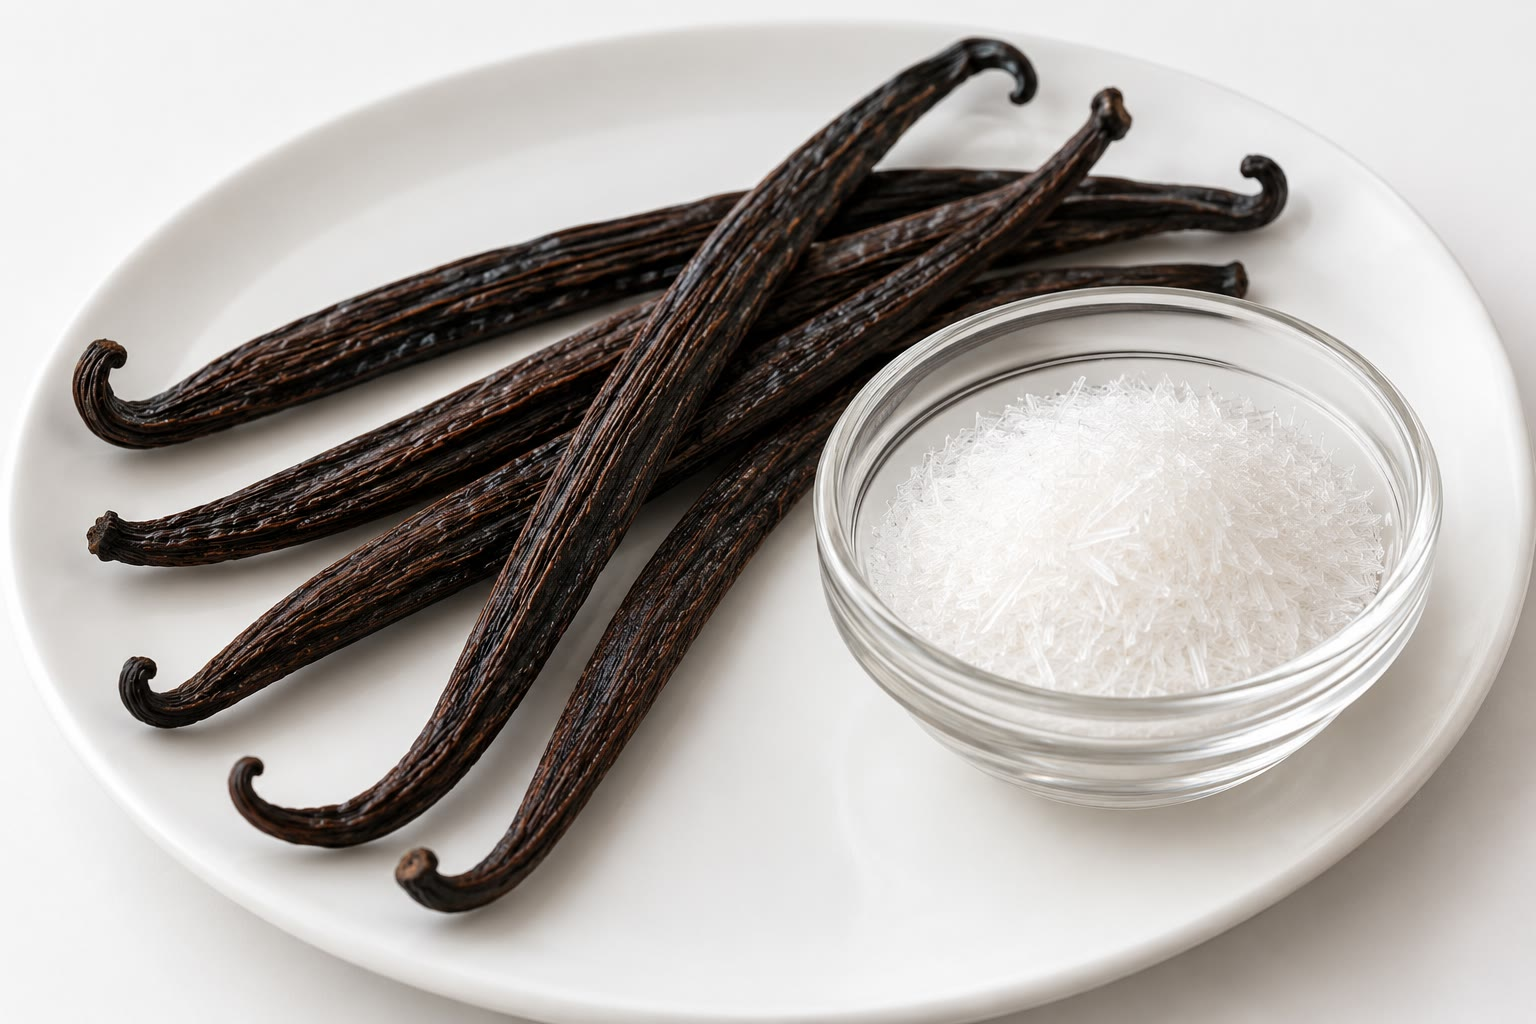
\includegraphics[width=0.55\linewidth]{images/book1/ai/g10-vanilla.jpg}

{\small Des gousses de vanille et des cristaux blancs de vanilline~: la
même \omterm{def:g7:atoms-and-molecules:molecule}{molécule}, venue d'une plante ou d'une usine.}
\end{omfigure}

\section{Espèces naturelles et espèces synthétiques}

\begin{definition}[Espèces naturelles et synthétiques]\label{def:g10:chemical-species:natural}
Une \emph{espèce naturelle}\index{espece naturelle@espèce naturelle} est une \omterm{def:g6:pure-substances-and-mixtures:species}{espèce
chimique} fabriquée par un être vivant ou présente telle quelle dans la
nature. Une \emph{espèce
synthétique}\index{espece synthetique@espèce synthétique} est fabriquée par les chimistes à
partir d'autres espèces, au moyen de \omterm{def:g7:chemical-reactions:reaction}{réactions chimiques}. Une espèce
synthétique peut être identique à une espèce naturelle (la vanilline de
synthèse) ou n'avoir aucun équivalent dans la nature (la plupart des
médicaments et des \omterm{def:g8:plastics:plastic}{matières plastiques}).
\end{definition}

\begin{proposition}[Même espèce, mêmes propriétés]\label{prop:g10:chemical-species:same}
Une \omterm{def:g6:pure-substances-and-mixtures:species}{espèce chimique} a les mêmes propriétés quelle que soit son origine~:
la vanilline fabriquée en usine et la vanilline extraite d'une gousse ont
la même formule, la même température de fusion, la même odeur. Ce qui
peut différer, c'est ce qui l'accompagne~: un extrait naturel est un
\omterm{def:g6:pure-substances-and-mixtures:mixture}{mélange}, qui contient beaucoup d'autres espèces modifiant son goût.
\end{proposition}

\begin{history}[De l'écorce de saule à l'aspirine, 1828--1899]
Pendant des siècles, on a mâché de l'écorce de saule contre la fièvre et
la douleur. En 1828, un chimiste en extrait l'espèce active, la
salicine~; les chimistes la transforment ensuite en acide salicylique,
efficace mais irritant pour l'estomac. En 1897, dans une entreprise de
colorants et de médicaments, Felix Hoffmann fabrique à partir de l'acide
salicylique une \omterm{def:g10:chemical-species:natural}{espèce synthétique} plus douce~: l'acide
acétylsalicylique, vendu à partir de 1899 sous le nom d'aspirine.
L'aspirine n'a aucune source naturelle~: c'est une espèce purement
synthétique.
\end{history}

\section{Extraire une espèce}

\begin{definition}[Extraction et extraction liquide--liquide]\label{def:g10:chemical-species:extraction}
Une \emph{extraction}\index{extraction} retire une \omterm{def:g6:pure-substances-and-mixtures:species}{espèce chimique} du
matériau qui la contient, en général en la dissolvant dans un \omterm{def:g6:solutions-and-solubility:solute}{solvant}
bien choisi. Lors d'une \emph{extraction liquide--liquide}\index{extraction liquide--liquide},
une espèce dissoute dans un liquide est transférée dans un second
liquide, \omterm{def:g6:solutions-and-solubility:miscible}{non miscible} avec le premier, dans lequel elle \omterm{def:g2:mixing-and-dissolving:dissolve}{se dissout}
mieux~; on sépare ensuite les deux liquides dans une ampoule à décanter.
\end{definition}

\begin{example}[Des extractions de tous les jours]\label{ex:g10:chemical-species:everyday}
Faire du thé est une \omterm{def:g10:chemical-species:extraction}{extraction} par l'eau chaude (infusion)~; faire
tremper des gousses de vanille dans l'alcool est une \omterm{def:g10:chemical-species:extraction}{extraction} par
l'éthanol (macération)~; faire bouillir des légumes pour préparer un
bouillon en est une autre (décoction).
\end{example}


\begin{definition}[Distillation et hydrodistillation]\label{def:g10:chemical-species:distillation}
Une \emph{distillation}\index{distillation} chauffe un \omterm{def:g6:pure-substances-and-mixtures:mixture}{mélange} liquide
jusqu'à l'ébullition, retransforme la vapeur en liquide dans un
réfrigérant parcouru par un courant d'eau froide, et recueille ce
liquide, le distillat. Une \emph{hydrodistillation}\index{hydrodistillation}
fait bouillir une matière végétale dans l'eau~: la vapeur d'eau entraîne
les espèces odorantes de la plante, qui se séparent de l'eau dans le
distillat sous forme d'une couche huileuse, l'huile essentielle.
\end{definition}

\begin{omfigure}
\begin{tikzpicture}[font=\small, scale=0.95]
  \pic[transform shape] at (0,0) {heatingmantle};
  \pic[transform shape] at (0,0) {rbflask={0.55}{omWater!70}};
  \foreach \x/\y in {-0.45/0.35,-0.1/0.55,0.3/0.3,0.5/0.7,-0.6/0.75,0.1/0.9,-0.25/0.2}
    \fill[green!45!black!70] (\x,\y) ellipse (0.09 and 0.04);
  \pic[transform shape] (s) at (0,3.0) {stillhead};
  \pic[transform shape] at ($(s-top)+(0,-0.75)$) {thermometer};
  \pic[transform shape, rotate=-20] (c) at (s-arm) {liebig={3.2}};
  \coordinate (cend) at ($(s-arm)+(-20:3.2)$);
  \pic[transform shape] (a) at (cend) {adapter};
  \pic[transform shape] at ($(a-tip)+(0,-2.3)$) {erlenmeyer={0.18}{omWater!70}};
  \fill[yellow!60!orange!60] ($(a-tip)+(-0.827,-2.3+0.47)$) -- ($(a-tip)+(0.827,-2.3+0.47)$) -- ($(a-tip)+(0.779,-2.3+0.6)$) -- ($(a-tip)+(-0.779,-2.3+0.6)$) -- cycle;
  \draw[<-, omProp, thick] (-0.55,0.55) -- (-2.2,0.9) node[left, text=black, align=right]
    {eau et fleurs\\ de lavande};
  \draw[<-, omProp, thick] (1.35,-0.6) -- (2.2,-1.1) node[right, text=black]
    {chauffe-ballon};
  \draw[<-, omProp, thick] (0.1,4.2) -- (-1.2,4.6) node[left, text=black] {thermomètre};
  \draw[<-, omProp, thick] ($(s-arm)+(-20:1.6)+(0,0.32)$) -- ++(0.6,1.0) node[above, text=black]
    {réfrigérant, parcouru par l'eau froide};
  \draw[<-, omProp, thick] ($(a-tip)+(0.4,-1.88)$) -- ++(1.1,0.2) node[right, text=black, align=left]
    {distillat~: huile essentielle\\ flottant sur l'eau};
\end{tikzpicture}

{\small \omterm{def:g10:chemical-species:distillation}{Hydrodistillation} de la lavande. La vapeur d'eau entraîne l'huile
essentielle dans le réfrigérant~; le distillat se sépare en une fine
couche d'huile au-dessus de l'eau.}
\end{omfigure}

\begin{method}[Choisir un solvant d'extraction]\label{met:g10:chemical-species:solvent}
Pour une \omterm{def:g10:chemical-species:extraction}{extraction liquide--liquide} d'une espèce dissoute dans l'eau,
le \omterm{def:g6:solutions-and-solubility:solute}{solvant} doit~:
\begin{enumerate}
  \item dissoudre l'espèce beaucoup mieux que l'eau~;
  \item être \omterm{def:g6:solutions-and-solubility:miscible}{non miscible} avec l'eau, pour que deux phases se forment~;
  \item être aussi peu dangereux que possible, et facile à éliminer
        ensuite (une basse température d'ébullition permet de
        l'évaporer).
\end{enumerate}
Ce sont les masses volumiques qui décident de la phase du dessus~: le
liquide le moins dense surnage.
\end{method}

\begin{example}[Des solvants pour l'huile de lavande]\label{ex:g10:chemical-species:table}
% ledger: rho:cyclohexane, bp:cyclohexane, rho:ethyl-acetate, bp:ethyl-acetate, rho:CH2Cl2, bp:CH2Cl2, rho:ethanol, bp:ethanol, sol:linalool
Le linalol, principale espèce de l'huile de lavande, ne \omterm{def:g2:mixing-and-dissolving:dissolve}{se dissout} qu'à
raison de \qty{1.6}{g/L} dans l'eau, mais très bien dans les \omterm{def:g6:solutions-and-solubility:solute}{solvants}
ci-dessous~:
\begin{center}
\small
\begin{tabular}{lccll}
\hline
\omterm{def:g6:solutions-and-solubility:solute}{solvant} & masse de \qty{1}{mL} & bout à & avec l'eau & principaux dangers \\
\hline
cyclohexane & \qty{0.78}{g} & \qty{81}{\celsius} & \omterm{def:g6:solutions-and-solubility:miscible}{non miscible} & inflammable, nocif \\
éthanoate d'éthyle & \qty{0.90}{g} & \qty{77}{\celsius} & \omterm{def:g6:solutions-and-solubility:miscible}{non miscible} & inflammable, irritant \\
dichlorométhane & \qty{1.33}{g} & \qty{40}{\celsius} & \omterm{def:g6:solutions-and-solubility:miscible}{non miscible} & cancérogène suspecté \\
éthanol & \qty{0.79}{g} & \qty{78}{\celsius} & \omterm{def:g6:solutions-and-solubility:miscible}{miscible} & inflammable \\
\hline
\end{tabular}
\end{center}
L'éthanol ne convient pas~: il se \omterm{def:g6:pure-substances-and-mixtures:mixture}{mélange} à l'eau et aucune phase ne se
forme. Avec le cyclohexane ou l'éthanoate d'éthyle, la phase du \omterm{def:g6:solutions-and-solubility:solute}{solvant}
est au-dessus~; avec le dichlorométhane, au-dessous.
\end{example}

\begin{omfigure}
\begin{tikzpicture}[font=\small, scale=1.2]
  \pic[transform shape] at (0,0) {sepfunnel={omWater!70}{yellow!35!orange!35}};
  \draw[<-, omProp, thick] (0.55,2.1) -- (1.6,2.4) node[right, text=black, align=left]
    {cyclohexane et huile\\ (moins dense, au-dessus)};
  \draw[<-, omProp, thick] (0.55,1.3) -- (1.6,1.2) node[right, text=black, align=left]
    {eau, évacuée\\ par le robinet};
  \draw[<-, omProp, thick] (0.25,0.52) -- (1.6,0.4) node[right, text=black] {robinet};
\end{tikzpicture}

{\small Une ampoule à décanter après agitation et \omterm{def:g3:separating-mixtures:decant}{décantation}~: l'huile
est passée dans le cyclohexane, au-dessus.}
\end{omfigure}

\begin{safety}{\ghs[0.8cm]{GHS02}\ghs[0.8cm]{GHS07}\ghs[0.8cm]{GHS08}\ghs[0.8cm]{GHS09}}
% ledger: ghs:cyclohexane
Le cyclohexane est très inflammable (GHS02)~; il peut être mortel en cas
d'ingestion et de pénétration dans les voies respiratoires, provoque une
irritation cutanée et de la somnolence (GHS07, GHS08)~; il est très
toxique pour les organismes aquatiques (GHS09). On l'utilise sous une
hotte, loin des flammes.
\end{safety}

\section{La chromatographie sur couche mince}

\begin{definition}[Chromatographie sur couche mince]\label{def:g10:chemical-species:tlc}
La \emph{chromatographie sur couche mince}\index{chromatographie sur couche mince}
(CCM) sépare les espèces d'un \omterm{def:g6:pure-substances-and-mixtures:mixture}{mélange} sur une plaque recouverte d'une
fine couche d'une poudre blanche, la \emph{phase stationnaire}\index{phase stationnaire}.
On dépose de petites taches des échantillons sur un trait de crayon
près du bas~; la plaque est placée dans une cuve fermée, dans un peu de
\omterm{def:g6:solutions-and-solubility:solute}{solvant}, l'\emph{éluant}\index{eluant@éluant}, qui monte le long de la plaque et
entraîne chaque espèce à une hauteur qui dépend de l'espèce. On révèle
ensuite les taches incolores, sous lumière ultraviolette ou avec des
vapeurs de diiode.
\end{definition}

\begin{definition}[Rapport frontal]\label{def:g10:chemical-species:retention-factor}
Le \emph{rapport frontal}\index{rapport frontal} d'une tache est
\[
  R_f = \frac{\text{distance de la ligne de dépôt à la tache}}
             {\text{distance de la ligne de dépôt au front du solvant}},
\]
un nombre compris entre 0 et 1. Pour une plaque, un \omterm{def:g10:chemical-species:tlc}{éluant} et une
température donnés, chaque espèce a son propre $R_f$.
\end{definition}

\begin{method}[Réaliser et lire une CCM]\label{met:g10:chemical-species:tlc}
\begin{enumerate}
  \item Tracer la ligne de dépôt au crayon à papier, à \qty{1}{cm} du
        bas~; y déposer une petite tache de chaque échantillon et de
        chaque espèce de référence.
  \item Placer la plaque dans la cuve, l'\omterm{def:g10:chemical-species:tlc}{éluant} sous la ligne~; fermer
        la cuve.
  \item Sortir la plaque quand le front est à environ \qty{1}{cm} du
        haut~; marquer aussitôt le front~; sécher et révéler.
  \item Mesurer les distances et calculer le $R_f$ de chaque tache. Un
        échantillon qui donne une seule tache est probablement une espèce
        pure~; une tache à la même hauteur qu'une tache de référence sur
        la même plaque correspond probablement à cette espèce.
\end{enumerate}
\end{method}

\begin{omfigure}
\begin{tikzpicture}[font=\small, scale=1.25]
  % the tank
  \pic[transform shape] at (0,0) {beaker={0.15}{omWater!80}};
  \fill[white] (-0.55,0.08) rectangle (0.55,1.92);
  \fill[omWater!80] (-0.55,0.08) rectangle (0.55,0.3);
  \draw[omGlass, line width=0.6pt] (-0.55,0.08) rectangle (0.55,1.92);
  \draw[black!60] (-0.55,0.42) -- (0.55,0.42);
  \foreach \x in {-0.3,0,0.3} \fill[black!70] (\x,0.42) circle (0.04);
  \fill[black!25] (-1.0,2.08) rectangle (1.0,2.18);
  \node[anchor=north, align=center] at (0,-0.15) {la cuve, fermée\\ par un couvercle};
  % the developed plate
  \begin{scope}[xshift=4.2cm]
    \pic[transform shape] at (0,0) {tlcplate};
    \draw[black!50, dashed] (-0.7,2.8) -- (0.7,2.8);
    \fill[omDef!70] (-0.35,1.36) ellipse (0.1 and 0.07);
    \fill[omDef!70] (-0.35,2.2) ellipse (0.1 and 0.07);
    \fill[omDef!70] (0,1.36) ellipse (0.1 and 0.07);
    \fill[omDef!70] (0.35,2.2) ellipse (0.1 and 0.07);
    \foreach \x/\l in {-0.35/O,0/L,0.35/A} \node[font=\footnotesize, anchor=north] at (\x,0.38) {\l};
    \draw[<->, omProp] (0.95,0.4) -- (0.95,1.36) node[midway, right, text=black, font=\footnotesize] {$d$};
    \draw[<->, omProp] (1.55,0.4) -- (1.55,2.8) node[midway, right, text=black, font=\footnotesize] {$D$};
    \draw[black!40, densely dotted] (-0.25,1.36) -- (0.95,1.36);
    \node[anchor=north, align=center] at (0.2,-0.15) {la plaque révélée~:\\ $R_f = d/D$};
  \end{scope}
\end{tikzpicture}

{\small CCM de l'huile de lavande (O) à côté du linalol (L) et de
l'éthanoate de linalyle (A). L'huile donne deux taches, aux hauteurs des
deux références~: elle contient les deux espèces. Pour le linalol,
$R_f = d/D$.}
\end{omfigure}

\section{Identifier une espèce par ses constantes physiques}

\begin{proposition}[La température de fusion vérifie l'identité et la pureté]\label{prop:g10:chemical-species:mp}
% ledger: mp:vanillin, mp:aspirin, mp:salicylic
Un solide pur fond nettement à une température qui lui est propre~: la
vanilline vers \qty{82}{\celsius}, l'aspirine à \qty{135}{\celsius},
l'acide salicylique à \qty{158}{\celsius}. Un échantillon impur fond plus
bas, et sur un intervalle de plusieurs degrés. Mesurer une température
de fusion, sur un banc Kofler ou dans un appareil de mesure du point de
fusion, permet donc à la fois d'identifier un solide et de savoir s'il
est pur.
\end{proposition}

\begin{inthelab}[Une plaque de CCM]
Les élèves déposent de l'huile de lavande, du linalol et de l'éthanoate
de linalyle sur une plaque, la développent dans un bocal fermé avec un
\omterm{def:g6:pure-substances-and-mixtures:mixture}{mélange} de \omterm{def:g6:solutions-and-solubility:solute}{solvants} choisi par l'enseignant, et la révèlent sous une
lampe ultraviolette, en portant des lunettes qui arrêtent les
ultraviolets. L'\omterm{def:g10:chemical-species:tlc}{éluant} est utilisé et manipulé sous la hotte.
\end{inthelab}

\begin{omfigure}
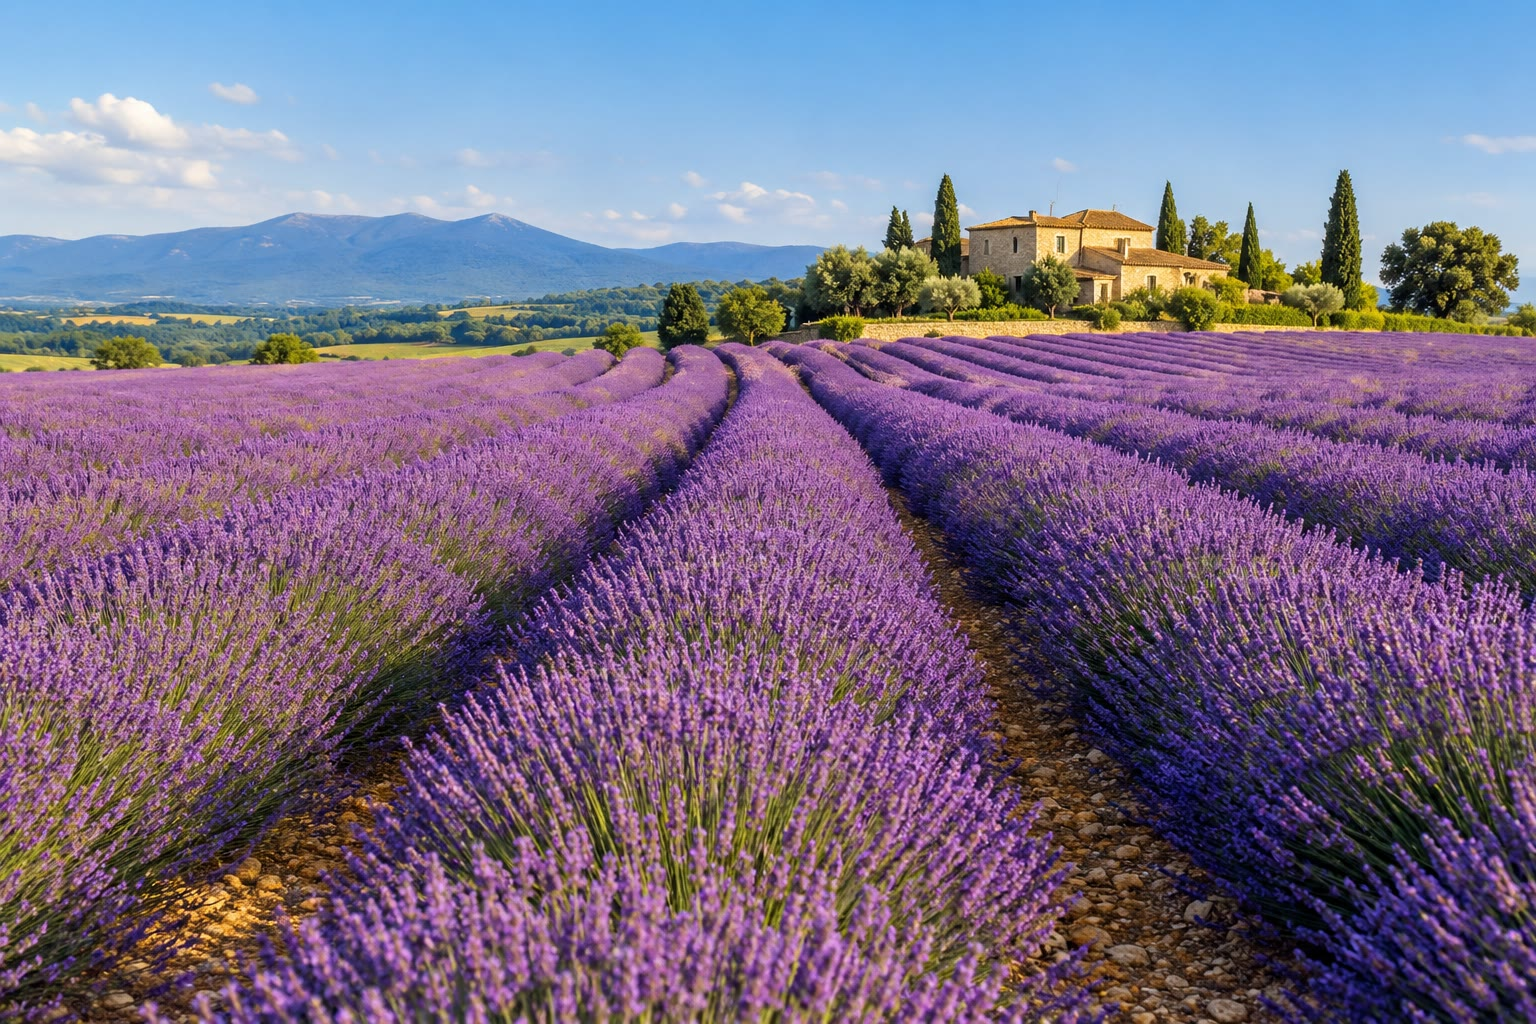
\includegraphics[width=0.55\linewidth]{images/book1/ai/g10-lavender-field.jpg}

{\small Un champ de lavande en fleur~: la \omterm{def:g5:raw-materials-and-recycling:raw-material}{matière première} de l'huile
essentielle de lavande.}
\end{omfigure}

\section{Exercices}

\begin{exercise}[$\star$]\label{exo:g10:chemical-species:1}
\omterm{def:g10:chemical-species:natural}{Espèce naturelle} ou synthétique~? La vanilline d'une gousse de vanille~;
l'aspirine~; la caféine des grains de café~; la vanilline fabriquée en
usine.
\end{exercise}

\begin{exercise}[$\star$]\label{exo:g10:chemical-species:2}
Expliquer pourquoi la vanilline de synthèse et la vanilline naturelle
ont la même température de fusion.
\end{exercise}

\begin{exercise}[$\star$]\label{exo:g10:chemical-species:3}
Sur une plaque de CCM, le front du \omterm{def:g6:solutions-and-solubility:solute}{solvant} est à \qty{6.0}{cm} au-dessus
de la ligne de dépôt et une tache à \qty{2.4}{cm}. Calculer son $R_f$.
\end{exercise}

\begin{exercise}[$\star$]\label{exo:g10:chemical-species:4}
Indiquer le rôle du réfrigérant dans une \omterm{def:g10:chemical-species:distillation}{distillation}, et expliquer
pourquoi l'eau froide entre par son extrémité inférieure.
\end{exercise}

\begin{exercise}[$\star$]\label{exo:g10:chemical-species:5}
Citer les trois conditions que doit remplir un \omterm{def:g6:solutions-and-solubility:solute}{solvant} d'\omterm{def:g10:chemical-species:extraction}{extraction}.
\end{exercise}

\begin{exercise}[$\star\star$]\label{exo:g10:chemical-species:6}
À l'aide du tableau des \omterm{def:g6:solutions-and-solubility:solute}{solvants}, expliquer pourquoi l'éthanol ne peut
pas servir à extraire le linalol du distillat, alors que le cyclohexane
le peut.
\end{exercise}

\begin{exercise}[$\star\star$]\label{exo:g10:chemical-species:7}
Dans une ampoule à décanter, on agite du dichlorométhane avec de l'eau.
Quelle phase est au-dessus~? Justifier à l'aide du tableau.
\end{exercise}

\begin{exercise}[$\star\star$]\label{exo:g10:chemical-species:8}
Une poudre blanche vendue comme de l'aspirine commence à fondre à
\qty{126}{\celsius} et est entièrement fondue à \qty{132}{\celsius}. Que
peut-on en conclure~?
\end{exercise}

\begin{exercise}[$\star\star$]\label{exo:g10:chemical-species:9}
Observer la figure de CCM de ce chapitre. Que contient l'huile de
lavande~? Quelle espèce est montée le plus haut~?
\end{exercise}

\begin{exercise}[$\star\star$]\label{exo:g10:chemical-species:10}
Remettre dans l'ordre les étapes de l'obtention de l'huile de lavande au
laboratoire~: séparation des phases~; \omterm{def:g10:chemical-species:distillation}{hydrodistillation}~; ajout de
cyclohexane au distillat et agitation~; \omterm{def:g3:separating-mixtures:evaporate}{évaporation} du cyclohexane.
\end{exercise}

\begin{exercise}[$\star\star$]\label{exo:g10:chemical-species:11}
Expliquer pourquoi la ligne de dépôt d'une plaque de CCM est tracée au
crayon à papier et placée au-dessus de l'\omterm{def:g10:chemical-species:tlc}{éluant}.
\end{exercise}

\begin{exercise}[$\star\star\star$]\label{exo:g10:chemical-species:12}
Après l'\omterm{def:g10:chemical-species:extraction}{extraction}, on élimine le cyclohexane en chauffant doucement, et
l'huile reste. À l'aide des températures d'ébullition du cyclohexane et
du linalol (\qty{198}{\celsius}), expliquer pourquoi cela fonctionne.
\end{exercise}

\begin{exercise}[$\star\star\star$]\label{exo:g10:chemical-species:13}
Un échantillon synthétique d'un arôme donne une seule tache sur une
plaque de CCM, à la hauteur de l'\omterm{def:g10:chemical-species:natural}{espèce naturelle}, et fond nettement à
la bonne température. Quelles conclusions peut-on en tirer~?
\end{exercise}

\begin{exercise}[$\star\star\star$]\label{exo:g10:chemical-species:14}
Sur la même CCM, la tache A a un $R_f = 0.40$ et le front est à
\qty{5.5}{cm} au-dessus de la ligne. À quelle hauteur se trouve la tache
A~? Une autre espèce a un $R_f = 0.75$~: à quelle distance au-dessus de
la tache A se trouve-t-elle~?
\end{exercise}

\begin{exercise}[$\star\star\star$]\label{exo:g10:chemical-species:15}
\qty{1.6}{g} de linalol peuvent \omterm{def:g2:mixing-and-dissolving:dissolve}{se dissoudre} dans \qty{1}{L} d'eau. Un
distillat de \qty{200}{mL} d'eau contient \qty{0.20}{g} de linalol
dissous. Est-il saturé~? Combien pourrait-il encore en dissoudre~?
Expliquer pourquoi il vaut la peine d'extraire cette eau au cyclohexane
plutôt que de la jeter.
\end{exercise}

\clearpage % garde le titre avec l'encadré de son problème (il était resté seul en bas de page)
\section{Problème~: le parfum de la lavande}

\begin{problem}[{Problème du week-end --- d'un panier de fleurs de lavande
à quelques gouttes d'huile essentielle, contrôlées par chromatographie}]
\label{pb:g10:chemical-species:1}
% ledger: rho:cyclohexane, bp:cyclohexane, rho:CH2Cl2, bp:linalool, ghs:cyclohexane
Dans un laboratoire de lycée, on hydrodistille \qty{100}{g} de fleurs
de lavande fraîches avec de l'eau. Le distillat, trouble, est agité avec
\qty{20}{mL} de cyclohexane dans une ampoule à décanter~; on garde la
phase de cyclohexane, on la sèche, puis on évapore le cyclohexane en
chauffant doucement. Ce qui reste est l'huile essentielle de lavande. On
utilisera le tableau des \omterm{def:g6:solutions-and-solubility:solute}{solvants} de ce chapitre.

\medskip
\noindent\textbf{Partie I --- L'\omterm{def:g10:chemical-species:distillation}{hydrodistillation}.}
\begin{enumerate}
  \item Quel est le rôle de l'eau bouillante dans une \omterm{def:g10:chemical-species:distillation}{hydrodistillation}~?
  \item Quel est le rôle du réfrigérant~? Par où l'eau froide y
        entre-t-elle~?
  \item Le distillat présente une fine couche huileuse qui flotte sur
        l'eau. L'huile est-elle \omterm{def:g6:solutions-and-solubility:miscible}{miscible} avec l'eau~? Est-elle plus ou
        moins dense que l'eau~?
  \item Pourquoi ne se contente-t-on pas de verser le distillat pour
        récupérer l'huile~?
\end{enumerate}

\medskip
\noindent\textbf{Partie II --- L'\omterm{def:g10:chemical-species:extraction}{extraction}.}
\begin{enumerate}[resume]
  \item Pourquoi le cyclohexane est-il un \omterm{def:g6:solutions-and-solubility:solute}{solvant} adapté à cette
        \omterm{def:g10:chemical-species:extraction}{extraction}~?
  \item Pourrait-on utiliser l'éthanol à la place~? Expliquer.
  \item Après agitation et \omterm{def:g3:separating-mixtures:decant}{décantation}, la phase de cyclohexane est-elle
        au-dessus ou au-dessous~? Qu'en serait-il avec le
        dichlorométhane~?
  \item Donner deux précautions imposées par les pictogrammes du
        cyclohexane.
  \item Pourquoi peut-on évaporer le cyclohexane sans perdre le
        linalol, qui bout à \qty{198}{\celsius}~?
\end{enumerate}

\medskip
\noindent\textbf{Partie III --- La chromatographie.}
On dépose l'huile, du linalol pur (L) et de l'éthanoate de linalyle pur
(A) sur une plaque de CCM. Après élution, le front est à \qty{6.0}{cm}
au-dessus de la ligne de dépôt. L'huile donne deux taches, à
\qty{2.4}{cm} et à \qty{4.5}{cm}~; la tache L est à \qty{2.4}{cm}, la
tache A à \qty{4.5}{cm}.
\begin{enumerate}[resume]
  \item Calculer le $R_f$ du linalol et celui de l'éthanoate de linalyle.
  \item Que contient l'huile, d'après cette plaque~?
  \item L'huile de lavande est-elle un \omterm{def:g6:pure-substances-and-mixtures:pure-substance}{corps pur}~?
  \item Pourquoi a-t-on déposé les références sur la même plaque que
        l'huile~?
  \item On dépose un linalol de synthèse sur une autre plaque éluée dans
        les mêmes conditions~: sa tache a un $R_f = 0.40$. Que peut-on en
        conclure~?
\end{enumerate}

\medskip
\noindent\textbf{Partie IV --- Combien d'huile~?}
L'huile obtenue occupe \qty{1.0}{mL}~; \qty{1}{mL} de cette huile pèse
\qty{0.90}{g}.
\begin{enumerate}[resume]
  \item Quelle masse d'huile a-t-on obtenue~?
  \item Quel pourcentage de la masse des fleurs cela représente-t-il~?
  \item Quelle masse de fleurs faudrait-il pour obtenir \qty{100}{g}
        d'huile~?
  \item On dit de cette huile qu'elle est «~naturelle~». En quel sens
        est-ce vrai~? Son linalol est-il différent du linalol de
        synthèse~?
  \item Donner la masse d'huile essentielle obtenue à partir de
        \qty{100}{g} de fleurs.
\end{enumerate}
\end{problem}
